\chapter{Architecture at Hybris}\label{chapter:hybris_architecture}
\section{Overview}\label{section:hybris_architecture/overview}
SAP \acrshort{YaaS} provides a variety of business services to support as well as enhance the products offered as SAP hybris front office such as hybris Commerce, hybris Marketing, hybris Billing etc. Using these offered services, developers can create their own business services focussed on their customer requirements.\\
The figure \ref{fig:hybris_architecture/overview/yaas_overview} provides the overview of \acrshort{YaaS}. \acrshort{YaaS} provides various business processes as a service (bPaaS) essential to develop applications and services thus filling up the gap between SaaS and HCP. For that purpose, it consumes the application services (aPaaS) provided by \acrshort{HCP}.
\begin{figure}[H]
\begin{center}
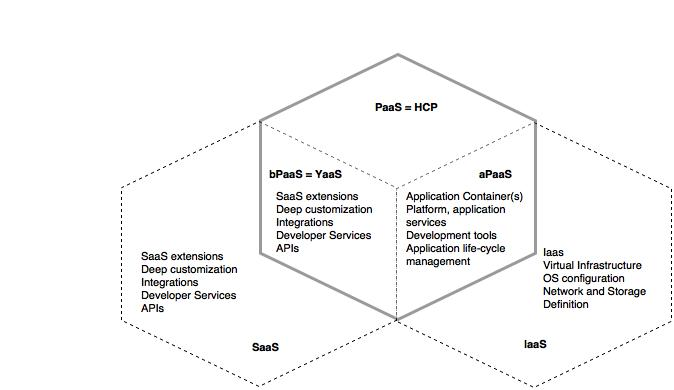
\includegraphics[width=0.8\textwidth]{figures/hybris-architecture-one}
\caption{\acrshort{YaaS} and \acrshort{HCP} \cite{Hirsch:2015aa}}
\label{fig:hybris_architecture/overview/yaas_overview}
\end{center}
\end{figure}
\\
\section{Vision}\label{section:hybris_architecture/vision}
The vision of \acrshort{YaaS} can be clarified with the following statement.
\begin{shaded}
"A cloud platform that allows everyone to easily develop, extend and sell services and applications." \\
\cite{Stubbe:2015aa}
\end{shaded}
The vision can be broadly categorized into following objectives.\\
\begin{enumerate}
\item \textbf{Cloud First}\\
The different parts of the application need to be scaled independently.
\item \textbf{Autonomy}\\
The development teams should be able to develop their modules independent of other teams and able to freely choose the technology that fits the job.
\item \textbf{Retain Speed}\\
The new features should be able to be released as fast as possible.
\item \textbf{Community}\\
It should be possible for the components to be shared across internal and external developers.
\end{enumerate}
The definition of microservices \ref{tab:context/microservices_architecture_style/keywords_extracted_from_various_definitions_of_microservice} as well as the characteristics of microservices [ref] signifies clearly that microservices architecture can be a good fit for \acrshort{YaaS} architecture.
\section{YaaS Architecture Principles}\label{section:hybris_architecture/YaaS_architecture_principles}
The Agile Manifesto \cite{Beck:2011aa} provides various principles to develop a software in a better way. It focus on fast response to the requirement changes with frequent continous delivery of software artifacts with close collaboration of customer and self-organizing teams.\\
The Reactive Manifesto \cite{Boner:2014aa} lists various qualities of a reactive system which includes responsiveness, resilience, elasticity and asynchronous message passing. Loose coupling is highly focused.
Furthermore, the twelve factors from Heroku \cite{Wiggins:2012aa} provides methodology for minimizing time and cost to develop software applications as services. It emphasizes on scalability of applications, explicit declaration as well as isolation of dependencies among components, multiple continuous deployments from a single version controlled codebase with separate pipelines for build, release and run.\\
Finally, the microservices architecture provides techiques of developing an application as a collection of autonomous small sized services focused on single responsibility. [section \ref{section:context/microservices_architecture_style}] It focus on independent deployment capability of individual microservices and suggest to use lightweight mechanisms such as http for communication among services. Following the architecture offers various advantages not limited to individual independent scalability of each microservice, resilience by isolating failure in a component and technology heterogeneity among various development teams.\cite{Newman:2015aa}
Following the principles mentioned above, a list of principles are compiled to be used as a guidelines for creating microservices. The list of principles are listed below.
\begin{enumerated}
\item \textbf{Self-Sufficient Teams}\\
The teams have independence and freedom for any decision related to the design and development of their components. This freedom is balanced by the responsibility for the team to handle the complete lifecycle of their components including smooth running as well as performance in production and troubleshooting in case of any problems.
\item \textbf{Open Technology landscape}\\
The team have freedom to choose any technology that they believe fits the requirement. They are completely responsible for the quality of their product. This gives teams, ownership as well as satisfaction for their products.
\item \textbf{Release early, release often}\\
The agile manifesto and twelve factors from Heroku also focus on continuous delivery of product to the clients. This will decrease time of feedback and ultimately fast response to the feedback resulting in high customer satisfaction. The teams are responsible to create build and delivery pipeline for all available environments.
\item \textbf{Responsibility}\\
The teams are the only responsible groups to work directly with the customers on behalf of their products. They need to work on the feedback provided by the customers. It will increase the quality of the products and relationship with customers. All the responsibilities including scaling, maintaining, supporting and improving products are handled by respective teams.
\item \textbf{\acrshort{API}s first}\\
The \acrshort{API} is a contract between service and consumers. The decision regarding design and development is very important as it can be one of the greatest assets if good or else can be a huge liability if done bad. \cite{Bloch:2016aa} The articles \cite{Bloch:2016aa} and \cite{Blanchette:2008aa} list various characteristics of good \acrshort{API} including simplicity, extensibility, maintainability, completeness, small and focussing on single functionality. Furthermore, a good approach to develop \acrshort{API} is to first design iteratively before implementation in order to understand the requirement clearly. Another important aspect of a good \acrshort{API} among many is complete and updated documentation.
\item \textbf{Predictable and easy-to-use UI}\\
The user interfaces should be simple, consistent across the system and also consistent to various user friendly patterns.\cite{Sollenberger:2012aa} The articles \cite{Martin:2013aa} and \cite{Porter:2016aa} specify additional principles to be considered when designing user interfaces. A few of them includes providing clarity with regard to purpose, smart organization and respecting the expectation as well as requirements of customers.
\item \textbf{Small and Simple Services}
A service should be small and focused on cohesive functionalities. The concept closely relates to the single responsibility principle. \cite{Martin:2016aa} A good approach is to explicitly create boundaries around business capabilities.\cite{Newman:2015aa}
\item \textbf{Scalability of technology}
The choice of technologies should be cloud friendly such that the products can scale cost-efficiently and without delay. It is influenced by the elasticity principle provided by the reactive manifesto.\cite{Boner:2014aa}
\item \textbf{Design for failure}
The service should be responsive in the time of failure. It can be possible by containment and isolation of failure within each component. Similarly, the recovery should be handled gracefully without affecting the overal availability of the entire system. \cite{Boner:2014aa}
\item \textbf{Independent Services}
The services should be autonomous. Each service should be able to be deployed independently. The services should be loosely coupled, they could be changed independently of eachother. The concept is highly enforced by exposing functionalities via \acrshort{API}s and using lightweight network calls as only way of communication among services. \cite{Newman:2015aa}
\item \textbf{Understand Your System}
It is crucial to have a good understanding of problem domain in order to create a good design. The concept of domain driven design strongly motivates this approach to indentify individual autonomous components, their boundaries and the communication patterns among them. \cite{Newman:2015aa} Furthermore, it is also important to understand the expectations of consumers regarding performance and then to realize them accordingly. It is possible only by installing necessary operational capabilities such as continuous delivery, monitoring, scaling and resilience.
\end{enumerated}
 